\documentclass{subfiles}

\begin{document}


This section gives a practical and scientific insight about the acquire data. 



The Remote Sensing data used in this thesis were mainly collected from two areas: the New Forest UK and a RedGum forest in Australia. The New Forest dataset contains hyperpsectral images, discrete LiDAR and FW LiDAR, while for the RedGum area only FW LiDAR were provided. Nevertheless, the FW LiDAR from those areas were collected using different instruments and have a few differences. Clarifying of the difference the data is important.

    \begin{figure}[!htbp]
    	\centering
    	\includegraphics[width=\textwidth]{img/Data_n_Instruments}
    	\caption{Data and Instruments}
    	\label{fig:dataInstrumentsRelations}
    \end{figure}

    two organisation:
	1. Natural Environment Research Council’s Airborne Research and Survey Facility (NERC ARSF)
	2. Interpine Ltd Group () 
	
	1. used for the hyperspectral Alignment
	2. dead tree detection
	both for visualisations and optimisations of various data structures
	
	The sample data used for this thesis are provided by Natural Environment Research Council’s Airborne Research and Survey Facility (NERC ARSF). The datasets mainly used were scanned on the 8th of April in 2010 at New Forest in UK. For every flightline, two Airborne Remote Sensing datasets are given: 
	

	




    \section{Airborne LiDAR systems}
    
    The Airborne Leica ALS50-II LiDAR system emits laser beams from a plane and collects information from the  returned laser intensity. When the beam hits an object (i.e. the forest canopy), then some of it bounces back while the rest penetrates through the tree branches. The laser beam continuous to break and partially return to the sensor until it reaches the ground. The LiDAR systems records information from the backscattered laser. 

    
     As mentioned at Section \ref{Background}, there are two types of LiDAR data, the discrete and the FW. The discrete LiDAR records a few peak laser returns, while the FW LiDAR system digitises and records the enitre backscattered signal into equally spaced time intervals, the wave samples. By measuring the round trip time of the beam at each time interval, the positions of the wave samples are calculated \cite{Wanger2004}. The delivered data is a set of waveforms. Each waveform is formed with a number of wave samples and each wave sample is characterised by its reflected intensity and position. The intensity is laser intensity recorded during its time interval and the position is the geographical coordinates that corresponds to that time interval \ref{fig:DiscreteFWSystem}.
    
         \begin{figure}[!htbp]
         	\centering
         	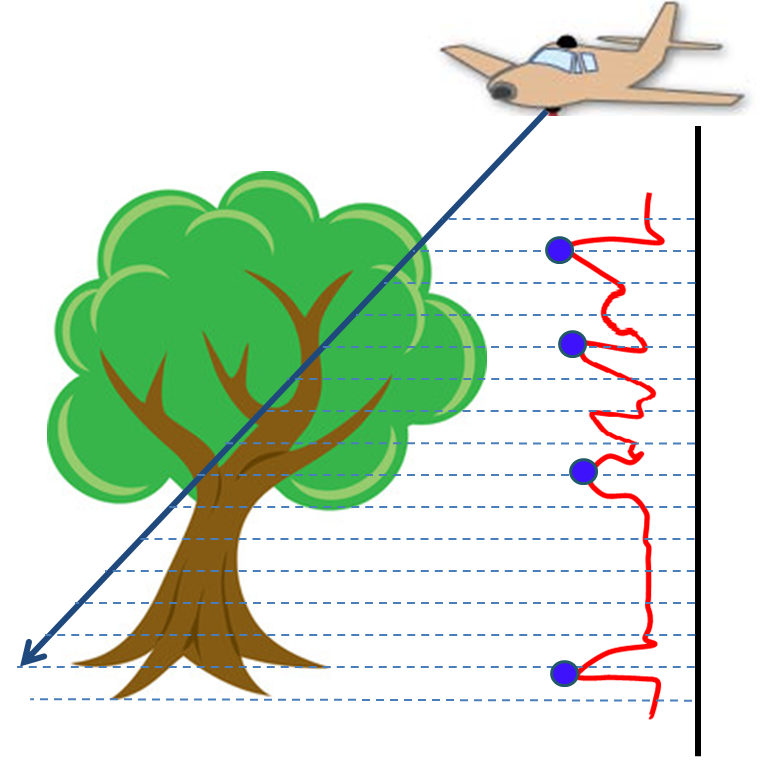
\includegraphics[width=\textwidth/3*2]{img/LiDAR_DiscretVsFW_fig}
         	\caption[Airborne LiDAR system]{Discrete and FW LiDAR data System \footnotemark}
         	\footnotetext{Tree image was retrieved from http://images.clipartpanda.com/tree-clip-art-Kij4jKriq.jpeg on 7th o f June. The plane image was retrieved form http://gmv.cast.uark.edu/wp-content/uploads/2013/01/         			 ALS\_scematic.jpg on the 6th of June} 
         	\label{fig:DiscreteFWSystem}
         \end{figure}
                 
        
         

	\section{Discrete LiDAR vs FW LiDAR}
    
   
   	
   	
   	The difference between the two sensors are further discussed in the following Sections

	\section{Leica Vs Trimble Instruments}
	
	
	\begin{table}[!htbp]
		
		\label{tab:InstrumentsSecifications}%
		\centering
		\begin{tabular}{|l||m{\textwidth/4}|m{\textwidth/4}|}
			\hline
			\textbf{Instrument Name:}	& \textbf{Leica ALS550-II}     & \textbf{Trimble Ax60  }    \\
			\hline\hline
			\textbf{Year of Introduction: }&Discrete LiDAR 2009 \& FW LiDAR 2010& 2013  \\
			\hline
			\textbf{Max Scan Frequency (kHz):} & 120 & 400  \\
			\hline
			\textbf{Recorded Intensity (bits):} & 8 & 16 \\
			\hline
			\textbf{Scanning Pattern:} & Sinusoidal  & The footprints are more equally spaced on the ground \\			
			\hline
			\textbf{Max field of view (degrees):} & 75 & 60	\\
			\hline
		\end{tabular}%
		\caption{Specifications of the LiDAR instruments used}
	\end{table}
	
	\par Nevertheless, the newest sensors RIEGL LMS-Q780 and RIEGL LMS-Q680i are native full-waveform sensors and the discrete LiDAR are produced by extracting peak points at post-processing. Therefore the concept of extracting a denser point clouds using Gaussian decomposition does not apply on data collected from those sensors. That was also proved by extracting peak points from RIEGL FW LiDAR data using the pulseextract from LAStools ~\cite{LAStools}. The number of points extracted was exactly the same as the number of points saved into the associated discrete LiDAR files.

	\section{Hyperspectral Imagery}
	\par Hyperspectral imagery has a positive impact in remote sensing because they contain information beyond human's visibility. The human eye receives light from the visual spectrum into three bands (red, green and blue). The hyperspectral sensors captures a larger spectrum and divides its light components into hundreds of bands, recording this way more information than a human eye can receive\cite{Smith2012}. 
	
	\par Nevertheless, raw airborne images  appear deformed because the pixel length varies across the flightline. NERC ARSF geo-corrects the data using the Airborne Processing Library (APL) \cite{Warren2014}. The processing levels are numbered. At 'level 3' the pixels are equally spaced and sized, but are slightly blurred. In this thesis, the 'level 1' data are used to preserve the highest possible quality. The 'level 1' data are non geo-corrected but they are associated with a file that defines the geographical location of each pixel. In practise, there are two files, the '.bil' and the '.igm'. The '.bil' file contains the hyperpsectral cube (Figure \ref{fig:hyperspectralCube}), all the pixel values at different wavelengths, and the .igm file gives the $x, y, z$ coordinates of each pixel.  
	
	\par The number of bands and the spectrum range captured depends on the hyperspectral sensor. The data from New Forest were collected using the following instruments:
	\begin{itemize}
		\item the Eagle, which captures the visible and near infra-red spectrum (400-970nm)
		\item the Haw, which covers short wave infra-red wavelengths(970-2450nm) 
	\end{itemize}
	Both sensors divide their spectrum range into 252 bands and each band is a 2D vector as shown in (Figure \ref{fig:hyperspectralCube}).
	
	\begin{figure}[!htbp]
		\centering
		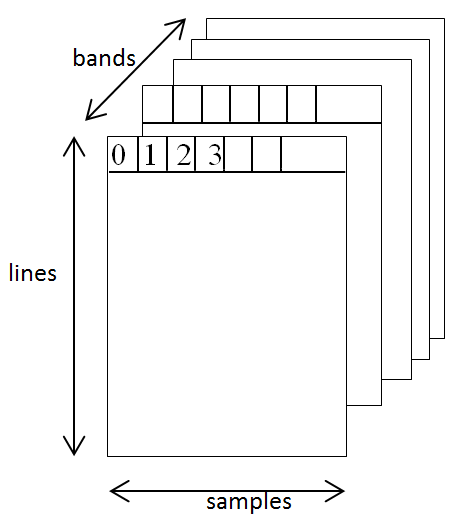
\includegraphics[width=\textwidth/5*2]{img/HI_bilFile}
		\caption[Hyperpsectral Cube]{This figure shows the order of the hyperspectral pixels saved into the the binary .bil file.}
		\label{fig:hyperspectralCube}
	\end{figure}
	
	By the way, the hyperpsectral images also come with a number of drawbacks. A few are mentioned here but since hyperpsectral imagery is not the main focused of the thesis there are not addressed:
	\begin{itemize}
		\item System faults sometimes occurs and the affected areas are masked out. This results into blank areas. 
		\item As a passive sensor, it is weather dependant and some areas are covered with clouds.
		\item Due to the high refraction of light at some wavelength, some bands are highly influenced by humidity (i.e. wavelength 1898.33).
	\end{itemize}
	
	To sum up, hyperpsectral images contain information beyond the visible and they are delivered into two file, one contains the hyperspectral cube and the other one the geo-locations of each pixel. In this project, they are used at chapter (Chapter \ref{Alignment}), where it is shown that the combination of Remote Sensing data confers better results for generating tree coverage maps. 
	
	
	
	
\end{document}